\documentclass{standalone}

\usepackage{tikz}
\usetikzlibrary{arrows}
\usetikzlibrary{arrows.meta}
\usetikzlibrary{positioning}
\usetikzlibrary{math}

% For correctly centering Dbar
\newlength{\dwidth}
\newlength{\shift}

\begin{document}
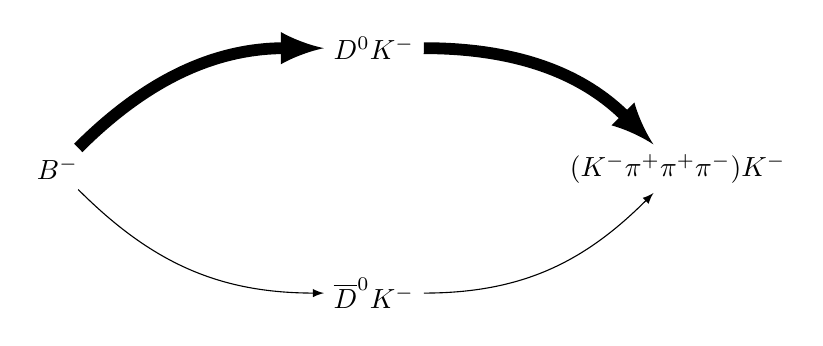
\begin{tikzpicture}
    \node (B) {$B^-$};

    \node (D) [above right=1cm and \shift+3cm of B] {$D^0K^-$};
    \node (Dbar) [below right=1cm and \shift+3cm of B] {$\overline{D}^0K^-$};
    \node (f) [right=6cm of B] {$(K^-\pi^+\pi^+\pi^-)K^-$};

    \draw[-latex, line width=1.5mm] (B) edge[out=45, in=180] node[above left] {} (D);
    \draw[-latex, line width=1.5mm] (D) edge[out=0, in=135] node[above right]{} (f);

    \draw[-latex] (B) edge[out=-45, in=180] node[below left]{} (Dbar);
    \draw[-latex] (Dbar) edge[out=0, in=-135] node[below right]{} (f);
\end{tikzpicture}
\end{document}

